\section{Grundlegende Definition und Eigenschaften}

\begin{df}\label{1.1}
Eine meromorphe Funktion $f : \mathbb{C} \to \hat{\mathbb{C}}:=\mathbb{C} \cup \lbrace\infty \rbrace$ heißt \textit{elliptisch} oder 
\textit{doppelperiodisch},
falls es Zahlen $\omega_1, \omega_2 \in \mathbb{C}$
mit $ \Im \nicefrac{\omega_1}{\omega_2} \neq 0$ gibt
und 
\begin{align*}
f(z+\omega_1) = f(z) = f(z+\omega_2) 
\end{align*}
für alle $z \in \mathbb{C}$ erfüllt ist.
\end{df}
\begin{figure}[h]
  \centering
    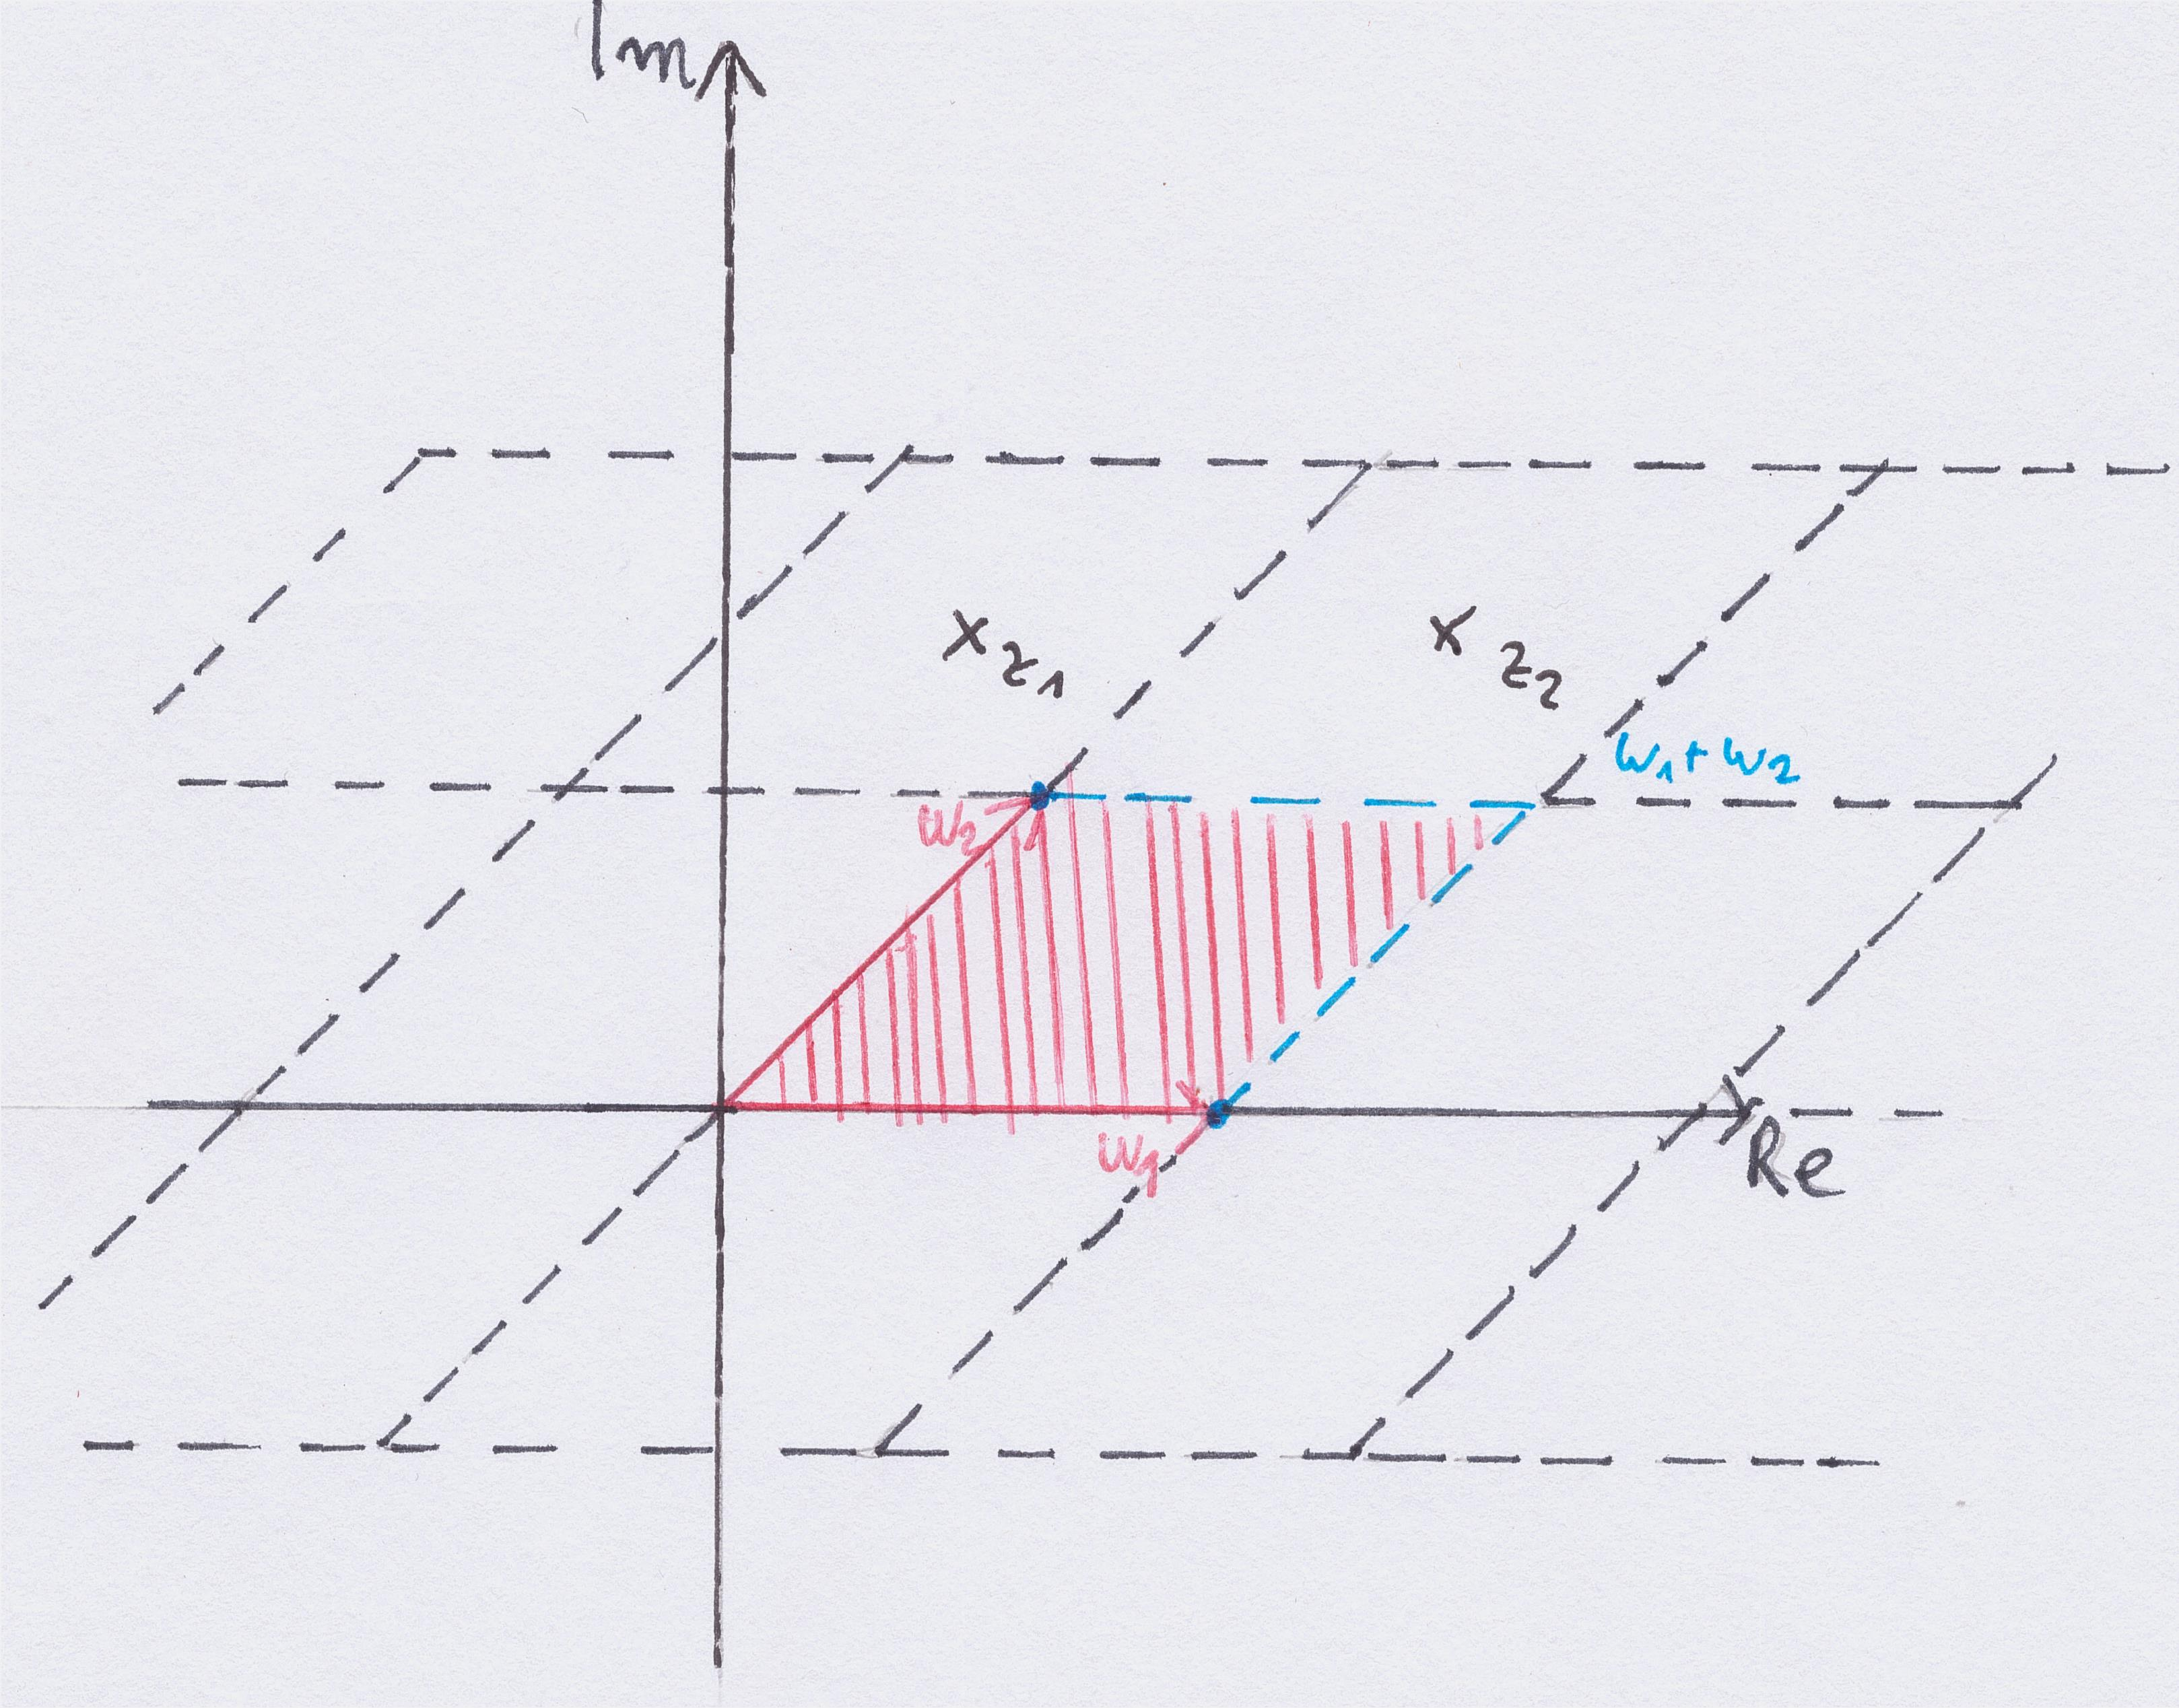
\includegraphics[width=0.65\textwidth]{sections/pics/Perioden}
  \caption{Beispiel eines Periodengitters}
\end{figure}
\begin{genericdef}{Periodenparallelogramm}\label{1.2}
Sei $f$ eine elliptische Funktion.
Das \textit{Periodengitter} von $f$ wird durch
\begin{align*}
\Gamma = \lbrace n \cdot \omega_1 + m \cdot \omega_2 \ | \ n,m \in \mathbb{Z} \rbrace
\end{align*}
beschrieben.
Da $\tau$ nicht reellwertig ist, spannen $\omega_1$ und $\omega_2$ ein Parallelogramm in der komplexen Ebene auf.
Zusätzlich setzt man $\Im \nicefrac{\omega_1}{\omega_2} < 0$ voraus,
damit die Eckpunkte $0$, $\omega_1$, $\omega_1+\omega_2$ und $\omega_2$ in einem positiven Sinn durchlaufen werden.
Nun besteht die Möglichkeit eine Äquivalenzrelation
\begin{align*}
z_1 \sim z_2 :\Leftrightarrow z_1-z_2 \in \Gamma
\end{align*}
zu definieren und die Funktion $f$ auf $\mathbb{C} / \Gamma$ zu betrachten.

Jede Äquivalenzklasse repräsentiert einen Punkt in dem aufgespannten Parallelogramm. Daraus erhält man, dass der blaue Teil des Randes nicht in dem Parallelogramm enthalten ist. Die Menge 
\begin{align*}
P := \lbrace  t \cdot \omega_1 + r \cdot \omega_2 \ | \ t,r \in [0,1) \rbrace
\end{align*} 
wird nun als \textit{Periodenparallelogramm} bezeichnet.
\begin{figure}[h]
  \centering
    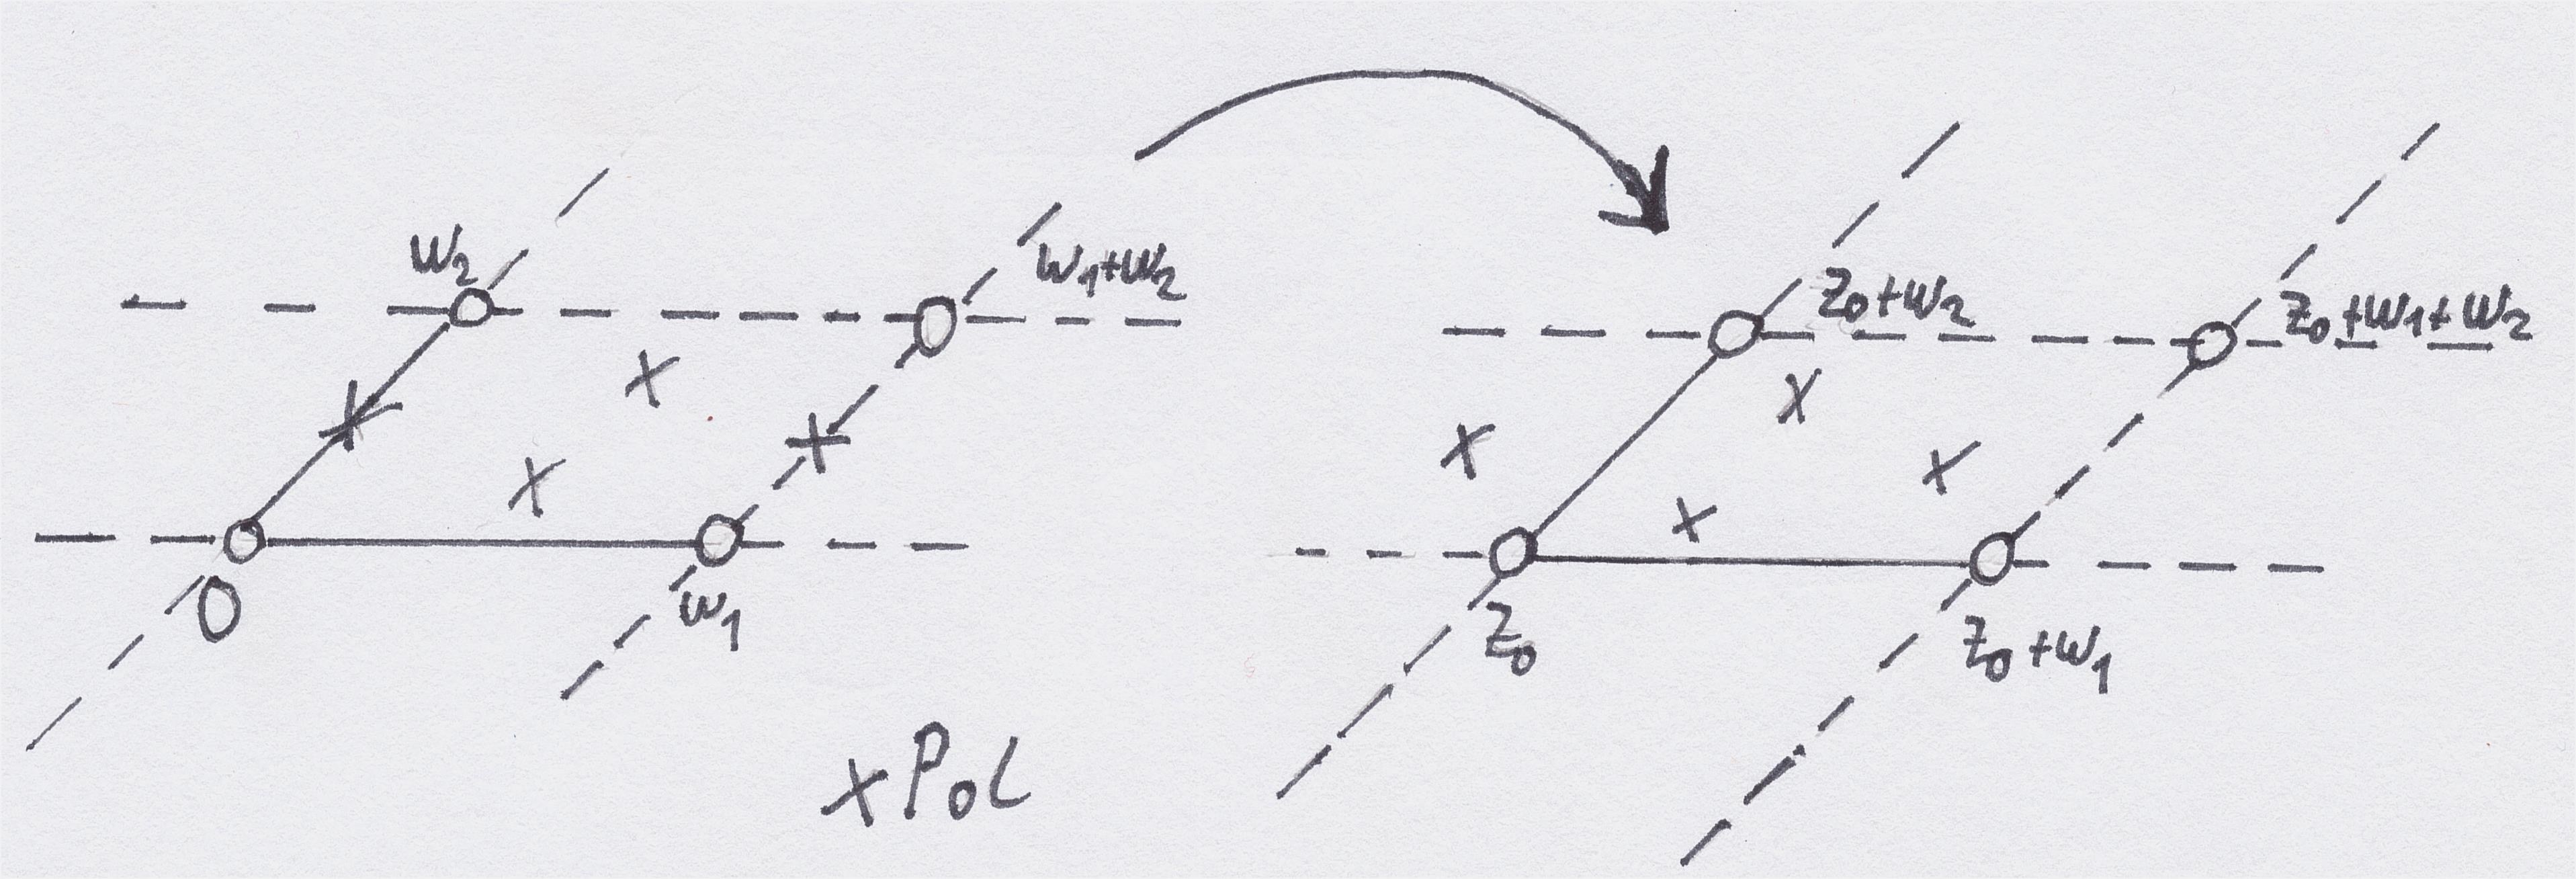
\includegraphics[width=0.80\textwidth]{sections/pics/verschiebung}
  \caption{Verschiebung}
\end{figure}
Für ein beliebiges $z_0 \in \mathbb{C}$
führt man mit
\begin{align*}
P_{z_o} := \lbrace z_0 + t \cdot \omega_1 + r \cdot \omega_2 \ | \ t,r \in [0,1) \rbrace
\end{align*}
eine \textit{Verschiebung des Periodenparallelogramms} ein.
Im weiteren Verlauf wird eine Eigenschaft oft innerhalb eines Periodenparallelogramms beschrieben. Dies bedeutet, dass eine Eigenschaft in einem beliebig verschobenen Periodenparallelogramm untersucht wird.
\end{genericdef}

\begin{df}\label{1.3}%Satz gefällt mir noch nicht.
Die \textit{Ordnung} $\ord(f)$ einer elliptischen Funktion $f$ ist die Anzahl der Pole unter Beachtung der Vielfachheit innerhalb eines Periodenparallelogramms.
\end{df}

\begin{sz}\label{1.4}
Seien $f,g,h$ elliptische Funktionen mit den Perioden $\omega_1, \omega_2$ und $ h\nequiv 0$ .
Dann sind $f + g$, $f \cdot g$, $\nicefrac{1}{h}$ und $f^\prime$ elliptische Funktionen mit den Perioden $\omega_1$ und $\omega_2$.
\end{sz}

\begin{proof}
%\begin{enumerate}[leftmargin=*]
%\item
Sei $z \in \mathbb{C}$ beliebig, wobei $z$ kein Pol von $f$ oder $g$ sein sollte.
Dann folgt sofort durch Nachrechnen:
\begin{align*}
(f+g)(z) = (f+g)(z+\omega_1)= (f+g)(z+\omega_2)
\end{align*}
Das Vorgehen ist für $f \cdot g$ und  $\nicefrac{1}{h}$ analog.
Bei $\nicefrac{1}{h}$ ist zu beachten, dass sich Null- und Polstellen vertauschen.
Man wird im weiteren Verlauf feststellen, dass dies die Ordnung nicht ändert.
%\item 
%Sei $z \in \mathbb{C}$ wieder beliebig und keine Polstelle von $f$.
Die Ableitung $f^\prime$ ist offenbar meromorph.
Weiter folgt mit der Identität aus Definition \ref{1.1} 
\begin{align*}
f^\prime(z+\omega_1) = f^\prime(z) = f^\prime(z+\omega_2) 
\end{align*}
und $f^\prime$ ist elliptisch.
%\end{enumerate}
\end{proof}

